\documentclass{standalone}
\usepackage{tikz}
\usetikzlibrary{patterns, angles}
\usepackage{circuitikz}

\begin{document}
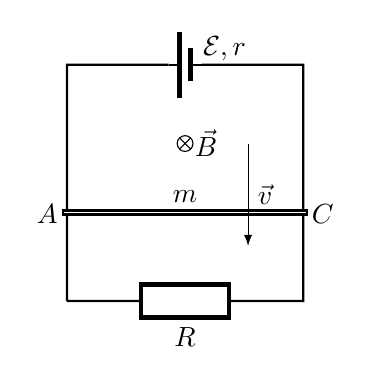
\begin{tikzpicture}[european] 
	\draw [thick] (0,-1) -- (0,2) to [battery1] (3,2) -- (3,-1) to [R=$R$] (0,-1);
	\node at (2.0,2.2) {$\mathcal{E}, r$};
	\node at (1.5,1) [right] {$\vec{B}$};
	\draw (1.5,1) circle (0.1);
	\draw (1.4293, 0.9293) -- (1.5707, 1.0707);
	\draw (1.4293, 1.0707) -- (1.5707, 0.9293);	
	\draw [thick, fill=white] (-0.05, 0.1) rectangle (3.05,0.15) node [above=0pt, midway] {$m$};
	\node at (-0.25,0.1) {$A$};
	\node at (3.25,0.1) {$C$};
	\draw [arrows={-latex}] (2.3,1)--(2.3,-0.3) node [midway, right] {$\vec{v}$};	
\end{tikzpicture}
\end{document}